%  LaTeX support: latex@mdpi.com 
%  For support, please attach all files needed for compiling as well as the log file, and specify your operating system, LaTeX version, and LaTeX editor.

%=================================================================
\documentclass[entropy,article,submit,pdftex,moreauthors]{Definitions/mdpi} 

%=================================================================
% MDPI internal commands - do not modify
\firstpage{1} 
\makeatletter 
\setcounter{page}{\@firstpage} 
\makeatother
\pubvolume{1}
\issuenum{1}
\articlenumber{0}
\pubyear{2024}
\copyrightyear{2024}
%\externaleditor{Academic Editor: Firstname Lastname}
\datereceived{ } 
\daterevised{ } % Comment out if no revised date
\dateaccepted{ } 
\datepublished{ } 
%\datecorrected{} % For corrected papers: "Corrected: XXX" date in the original paper.
%\dateretracted{} % For corrected papers: "Retracted: XXX" date in the original paper.
\hreflink{https://doi.org/} % If needed use \linebreak
%\doinum{}
%\pdfoutput=1 % Uncommented for upload to arXiv.org
%\CorrStatement{yes}  % For updates


%=================================================================
% Add packages and commands here. The following packages are loaded in our class file: fontenc, inputenc, calc, indentfirst, fancyhdr, graphicx, epstopdf, lastpage, ifthen, float, amsmath, amssymb, lineno, setspace, enumitem, mathpazo, booktabs, titlesec, etoolbox, tabto, xcolor, colortbl, soul, multirow, microtype, tikz, totcount, changepage, attrib, upgreek, array, tabularx, pbox, ragged2e, tocloft, marginnote, marginfix, enotez, amsthm, natbib, hyperref, cleveref, scrextend, url, geometry, newfloat, caption, draftwatermark, seqsplit
% cleveref: load \crefname definitions after \begin{document}

%=================================================================
% Please use the following mathematics environments: Theorem, Lemma, Corollary, Proposition, Characterization, Property, Problem, Example, ExamplesandDefinitions, Hypothesis, Remark, Definition, Notation, Assumption
%% For proofs, please use the proof environment (the amsthm package is loaded by the MDPI class).

%=================================================================
% Full title of the paper (Capitalized)
\Title{How Information Evolves}

% MDPI internal command: Title for citation in the left column
\TitleCitation{How Information Evolves}

% Authors, for the paper (add full first names)
\Author{Dan Adler $^{1}$}

%\longauthorlist{no}

% MDPI internal command: Authors, for metadata in PDF
\AuthorNames{Dan Adler}

% MDPI internal command: Authors, for citation in the left column
\AuthorCitation{Dan Adler}
% If this is a Chicago style journal: Lastname, Firstname, Firstname Lastname, and Firstname Lastname.

% Affiliations / Addresses (Add [1] after \address if there is only one affiliation.)
\address{%
$^{1}$ \quad dan@danadler.com}

%\simplesumm{} % Simple summary

%\conference{} % An extended version of a conference paper

% Abstract (Do not insert blank lines, i.e. \\) 
\abstract{The emergence of complexity and information is a fundamental question spanning disciplines from physics to biology and computation. While traditional approaches describe information as an emergent property, they leave unresolved how complexity arises dynamically from purely abiotic processes. This paper presents ABC systems, an abstract framework that models the evolution of patterns through probabilistic interactions and stability-driven selection. By abstracting away specific physical laws, these systems demonstrate a universal mechanism for generating order and information. ABC systems evolve patterns over successive generations, with selection pressures favoring stable configurations that persist and interact more frequently. These dynamics have the potential to encode logic, computational rules, and, under certain conditions, self-replicating behaviors, thereby offering a conceptual pathway to better understand the transition from abiotic to biotic evolution. However, substantial work remains to demonstrate these principles in realistic prebiotic scenarios or computational analogs. The framework also highlights the interplay between top-down and bottom-up causality, illustrating how emergent patterns recursively influence their formation while being shaped by local interactions. This study offers a computationally realizable pathway that may help bridge randomness and complexity. By illustrating a potential link among entropy reduction, emergent computation, and dynamic information storage, it highlights how certain abstract systems could, in principle, transition from disordered states toward more ordered, information-rich configurations. Further empirical validation and more detailed modeling are needed to confirm and refine these suggestions.
}

% Keywords
\keyword{Abiotic evolution; Emergent complexity; Information dynamics; Stability-driven selection; Top-down causality; Bottom-up causality; Cellular automata; Bayesian updating; Entropy reduction; Probabilistic interactions; Computational emergence; Prebiotic systems}


\graphicspath{{images/}}

%%%%%%%%%%%%%%%%%%%%%%%%%%%%%%%%%%%%%%%%%%
\begin{document}
%%%%%%%%%%%%%%%%%%%%%%%%%%%%%%%%%%%%%%%%%%

% The order of the section titles is different for some journals. Please refer to the "Instructions for Authors” on the journal homepage.

\section{Introduction}

The study of evolution, complexity, and information has been a cornerstone of multiple scientific disciplines that bridge physics, biology, and computation. Foundational works such as Schrödinger's \textit{What is Life?} \cite{schrodinger1944life} posed fundamental questions about how order emerges from disorder, inspiring theoretical explorations of how physical laws govern the emergence of biological systems. Tegmark's \textit{Mathematical Universe Hypothesis} \cite{tegmark2008mathematical} posits that the universe itself is a mathematical structure, where physical phenomena are manifestations of abstract mathematical rules. These works frame the question of complexity, but leave the mechanisms of emergence unaddressed.

In the realm of evolutionary dynamics, Fisher \cite{fisher1930genetical} and Nowak \cite{nowak2006evolutionary} provide mathematical models that describe the mechanisms of replication, mutation, and selection. Although these models illuminate the principles of biological evolution, they assume the existence of self-replicating, mutating entities and do not delve into how such entities might arise from purely abiotic processes. Similarly, Wheeler's concept of "It from Bit" \cite{wheeler1990itbit} intriguingly suggests that information underpins the physical world, but it lacks a concrete mechanism for how information structures form and evolve.

Dennis Noble's work on top-down causality \cite{noble2012causality} emphasizes the role of systems-level behavior in determining lower-level interactions. This perspective challenges reductionist paradigms, but does not address how such systems might emerge from simpler abiotic conditions. On the computational side, Seth Lloyd’s concept of the universe as a quantum computer \cite{lloyd2006programming} provides a framework for understanding the universe as a computational entity but leaves open the question of how specific computational rules or patterns arise.

Algorithmic complexity \cite{kolmogorov1965complexity} \cite{chaitin1977algorithmic} \cite{solomonoff1964formal} and Shannon’s information theory \cite{shannon1948mathematical} provide powerful tools to quantify information and complexity, but do not explain how information is created or evolves within physical systems. These frameworks focus on static measures of complexity, often missing the dynamic interplay between interactions and selection that drives the formation of ordered structures.

This paper introduces "ABC systems" which offer an abstract model for the emergence of complexity and information. Unlike prior work tied to physical systems or abstract concepts without implementation pathways, ABC systems provide a plausible mechanism for how stable patterns might arise, evolve, and persist based solely on probabilistic interactions. Although ABC systems abstract away specific physics, they propose a general conceptual framework that may be adaptable to diverse scenarios, from chemical interactions to computational models. Future work will be required to rigorously connect these abstractions to concrete experimental or simulated systems.

In contrast to Deutch \& Marletto's Constructor Theory \cite{deutsch2013constructor}, which lacks a generative mechanism, ABC systems demonstrate how information structures emerge dynamically through selection pressures. Unlike evolutionary dynamics as formulated by Nowak, which assumes preexisting replicators, ABC systems show how stable, self-replicating patterns can arise from purely abiotic interactions. Furthermore, the framework of ABC systems provides a path to connect the abstract ideas of Lloyd and Tegmark with practical, realizable dynamics, where probabilistic interactions evolve into ordered patterns encoding information.

\section{ABC System Fundamentals}

We define "ABC Systems" as follows: a population of elements \( A, B, C, \dots \) capable of forming compounds through local interactions of unspecified forces. These elements could exist in our physical universe, or in an abstract universe. The stability of compounds determines how many generations they will persist, and we assume that base elements dissipate and regenerate every generation. Over successive generations, the system undergoes a form of natural selection where compound stability drives the evolution of the population. ABC systems are governed by two distinct but interrelated probability distributions: The population distribution, reflecting the relative abundance of patterns in the system, and the stability distribution, representing the likelihood that interactions between patterns are successful and result in new, stable patterns. Together, these distributions determine the dynamics of the system, including the selection of stable patterns, their evolution over generations, and the emergent information encoded within the system.

Consider a simple population of 3 elements: {A, B, C}. Assume B-compounds are more stable than those without B. Thus AB, BC, ABC, have a higher stability than AC or A or C. Therefore, B-compounds will persist over multiple generations, while the others will quickly dissipate. The more stable B-compounds will interact more frequently due to their relative frequency, even without replication or inheritance. A simulation may look like this:

\begin{figure}[htp]
    \centering
    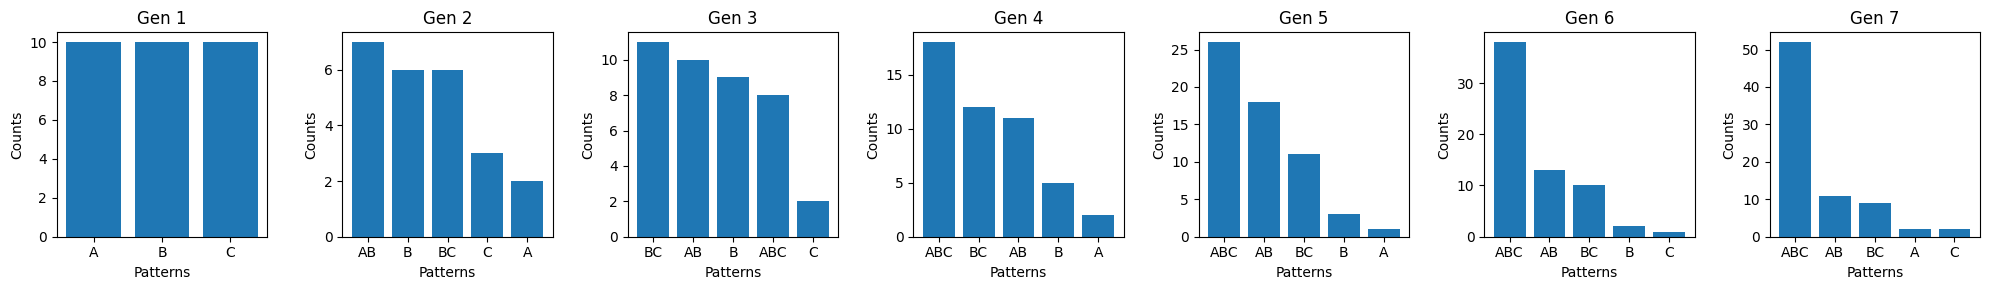
\includegraphics[width=13cm]{pat_1}
    \caption{ABC System population evolution simulation}
    \label{fig:pat_1}
\end{figure}

Where is Maxwell's demon \cite{leff2002maxwell} hiding in this example, driving it towards a low-entropy state? The answer lies in the roulette wheel. Compounds that persist longer have more chances to interact. As their frequency in the population grows, their chances to interact grow even more. In Evolutionary Dynamics, this is called fitness-proportionate selection \cite{back1996evolutionary} or roulette wheel selection \cite{goldberg1989genetic} \cite{holland1975adaptation}.

\section{Dual Probability Distributions Governing ABC Systems}

ABC systems can be effectively described by two interdependent probability distributions: the \textbf{population distribution}, which represents the relative abundance of patterns in the system, and the \textbf{stability distribution}, which quantifies the likelihood of successful interactions between patterns and the resulting stability of those interactions. These distributions interact to drive the system's dynamics, determining which patterns persist, dominate, or dissipate over time.

The population distribution reflects the probabilities of patterns at any given generation \( t \). Let \( P(p_t) \) represent the probability of pattern \( p \) in the population at time \( t \):
\[
P(p_t) = \frac{N(p_t)}{\sum_{q \in P} N(q_t)},
\]
where \( N(p_t) \) is the absolute count of pattern \( p \) in the population at time \( t \), and \( \sum_{q \in P} N(q_t) \) is the total population size at time \( t \), ensuring normalization (\( \sum_{p \in P} P(p_t) = 1 \)). The population distribution evolves over generations as patterns interact and new stable configurations emerge. As patterns with higher stability and frequent interactions become more prominent in the population, the population distribution evolves to reflects the history of past interactions and selection pressures.

The stability distribution represents the probability of successful interactions between patterns \( p \) and \( q \). Let \( S(p, q) \) denote the stability of the interaction between \( p \) and \( q \), defined as:
\[
S(p, q) = P(r | p, q),
\]
where \( P(r | p, q) \) is the conditional probability of forming pattern \( r \) as a result of the interaction between \( p \) and \( q \).

Stability reflects inherent properties of patterns, such as physical proximity, strength of bonds, geometric compatibility, energy barriers, or interaction rules. Stability values vary for different pairs of patterns, which influences which interactions dominate the dynamics. Although the population distribution evolves rapidly, the stability distribution remains constant or changes only gradually.

\subsection{Combined Role of Population and Stability Distributions}

Together, the two distributions determine the dynamics of the system. The probability of two patterns \( p \) and \( q \) interacting to form a new pattern \( r \) is proportional to their population probabilities and the stability of their interaction:
\[
P(p_{t+1}) \propto P(p_t) \cdot \sum_{q \in P} P(q_t) \cdot S(p, q).
\]
The continuous-time dynamics of the feedback system can be derived as a natural extension of the discrete update equation:
\[
\frac{dP(p, t)}{dt} \propto \alpha P(p, t) \cdot S_{\text{eff}},
\]
where \( S_{\text{eff}} = \sum_{q \in P} P(q, t) \cdot S(p, q) \) is the effective stability of the pattern. Order is generated in the system through feedback-driven amplification of stable patterns. Solving this equation, we see that the probability of a pattern \( P(p, t) \) grows exponentially over time as a result of stabilizing interactions:
\[
P(p, t) \propto \exp(\alpha S_{\text{eff}} t),
\]
where \( \alpha \) is the growth rate constant, and \( S_{\text{eff}} \) is the effective stability of the pattern. This exponential growth rapidly increases the dominance of stable patterns in the population.

In contrast, random processes and stochastic fluctuations redistribute probabilities in the system, contributing to an increase in entropy. The degradation of order due to these random effects is characterized by a slower logarithmic growth in entropy:
\[
\Delta H \propto \ln(t).
\]
As time progresses, the competition between the exponential growth of stable patterns and the logarithmic increase in entropy becomes evident. The net result is that the exponential growth of order, driven by stabilizing feedback and represented as \( \exp(\alpha S_{\text{eff}} t) \), outpaces the entropy increase \( \ln(t) \). This ensures that stability-driven feedback creates a net reduction in entropy, leading the system toward a more ordered, low-entropy state. Over time, the dominance of stable patterns suppresses randomness, driving the system into configurations characterized by emergent complexity and order.

This analysis demonstrates how stability-driven interactions in local populations generate order faster than the second law of thermodynamics can degrade it. While random fluctuations tend to increase entropy, the exponential reinforcement of stable patterns creates a net reduction in entropy, leading to emergent order. The dynamics also highlight the competitive nature of the system: only patterns with sufficiently high stability and effective interaction networks survive over the long term, ensuring the self-organization of the population into ordered configurations.

\subsection{Defining Stability in ABC Systems}

In ABC systems, the \textit{stability} distribution determines which patterns persist and thus influence subsequent interactions. When compared to physical systems, stability may be defined as a product of three factors: longevity, interactivity, and environmental conditions:

\[
S(p, q) = Longevity \cdot Interactivity \cdot Environment
\]

Longevity measures how long a patterns endure, thus increasing its probability of participating in future interactions. For example, the stability of \(H_2O\) molecules stems from strong covalent bonds that allow them to persist and engage in subsequent reactions. Interactivity represents a pattern’s capacity to form new connections, analogous to valency in chemistry. Carbon’s high valence, for instance, enables it to create a wide array of stable compounds. Environmental Factors include temperature, pressure, and concentration, all of which influence how likely patterns are to form or persist. Ice formation depends on temperature and pressure, while higher reactant concentrations increase the likelihood of productive encounters.

\subsection{Catalysis}

Consider an ABC system where \( A \) interacts with \( B \) to form a compound \( AB \), but this interaction occurs only in the presence of a catalyst \( C \). The catalyst \( C \) is not consumed or altered during the interaction, yet it influences the system's dynamics by facilitating specific reactions. This creates selection pressure for \( C \) to persist due to its role in enabling the formation of stable compounds. In this case, the catalyst \( C \) facilitates the reaction by increasing its likelihood:
\[
P(A + B \to AB \mid C) \propto p_A \cdot p_B \cdot p_C.
\]

The catalyst \( C \) benefits indirectly, as its presence enables reactions that increase the overall fitness of the system. This means we can expect a higher probability of \( C \) in later generations, even though it does not directly form stable compounds.

\section{Mixing Two ABC Systems: Entropy Dynamics}

Mixing two independently evolved ABC systems introduces a new dimension to their dynamics, where patterns and interactions from each system influence the other. This interaction results in the exchange of information, changes in entropy, and the potential emergence of novel patterns. By analyzing information flow and entropy in such mixed systems, we can gain deeper insights into the dynamics of evolving systems and their capacity for self-organization.

Let two independently evolved ABC systems \( P_1 \) and \( P_2 \) represent populations of patterns \( \{A, B, C, \dots\} \) and \( \{X, Y, Z, \dots\} \), respectively. Each system evolves independently based on its population distribution \( P(p_t) \) and stability constraints \( S(p, q) \) for patterns \( p, q \) within the same system.

When the two systems are mixed, the patterns from \( P_1 \) and \( P_2 \) interact, allowing the formation of cross-system compounds (e.g., \( ABX, BYZ \)). Stability constraints extend to cross-system interactions, introducing new terms \( S(p, q) \) where \( p \in P_1 \) and \( q \in P_2 \). The joint system evolves based on updated probabilities reflecting both within-system and cross-system interactions.

\begin{figure}[htp]
    \centering
    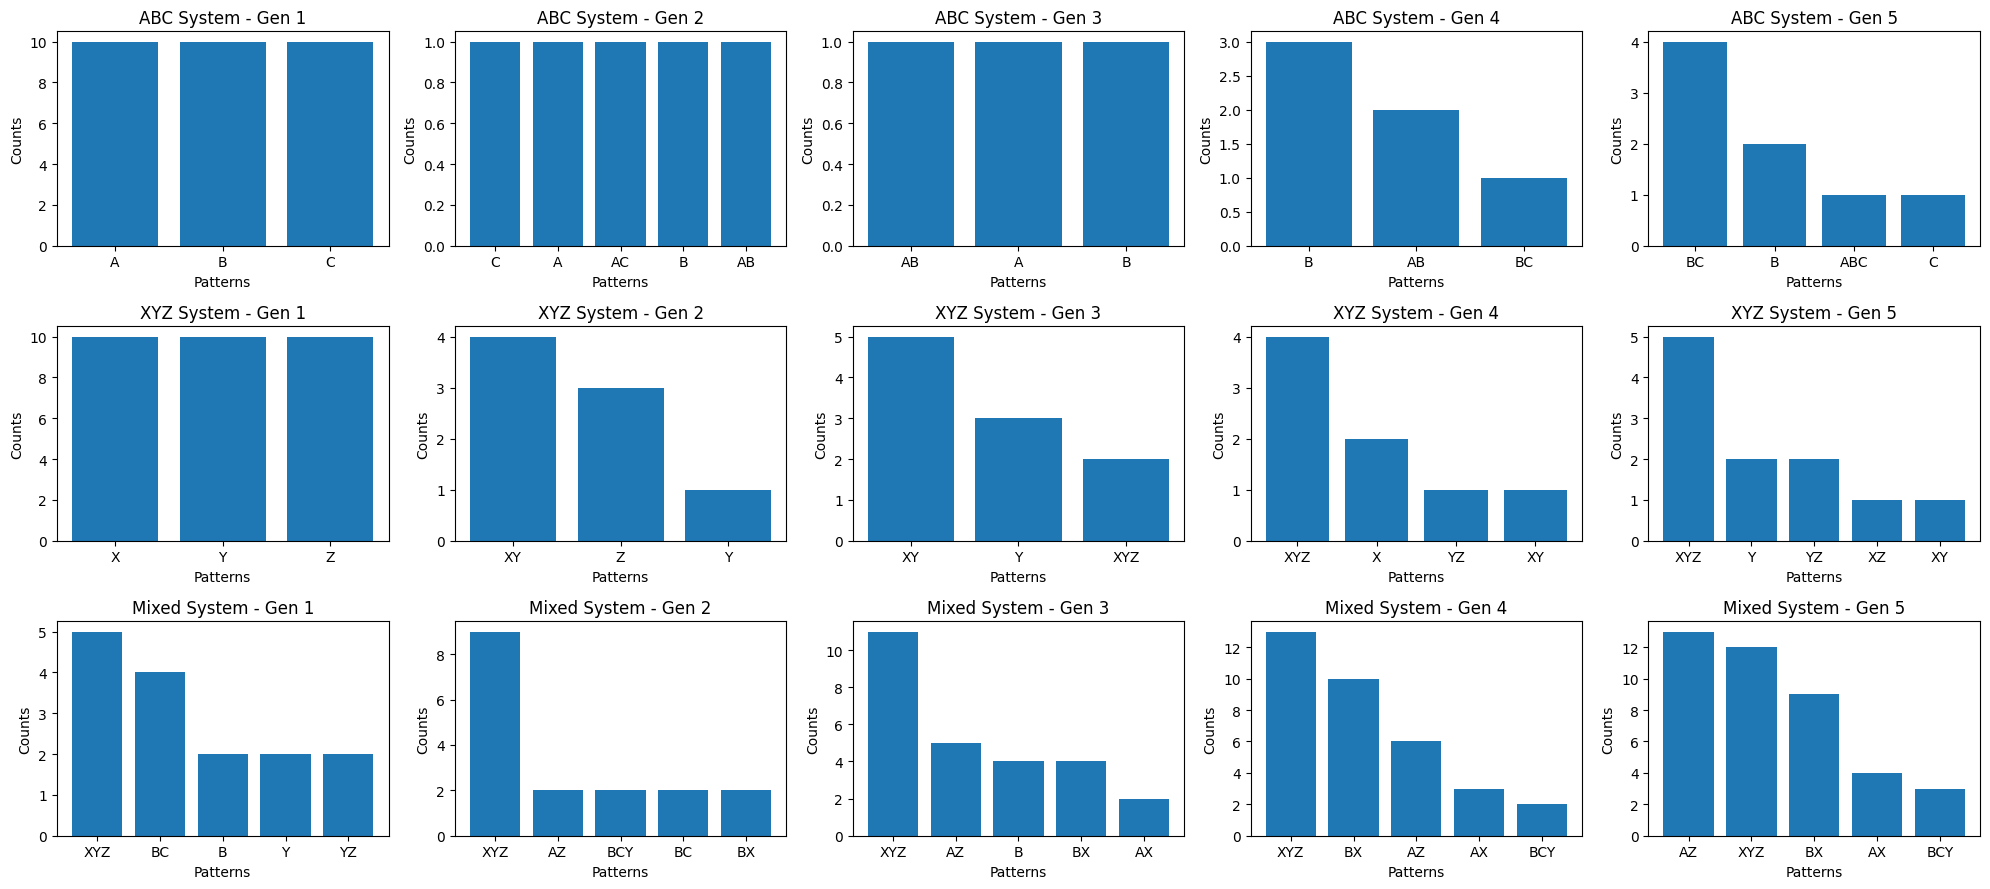
\includegraphics[width=13cm]{mixed_1}
    \caption{Mixing two evolved populations}
    \label{fig:mixed_1}
\end{figure}

\subsection{Entropy Dynamics in Mixed Systems}

After mixing, the joint entropy \( H_{\text{mix}}(t) \) becomes:
\[
H_{\text{mix}}(t) = -\sum_{p \in P_1 \cup P_2} P(p_t) \ln P(p_t),
\]
where \( P(p_t) \) now includes probabilities of cross-system patterns.

If both \( P_1 \) and \( P_2 \) are in low-entropy states, characterized by dominance of stable patterns, the mixed system is likely to retain a low entropy. The interaction of well-organized patterns results in selective formation of cross-system compounds, reinforcing order.

If either \( P_1 \) or \( P_2 \) has high entropy, the mixing introduces randomness into the more ordered system. Cross-system interactions may lead to transient increases in entropy, but selection pressures favoring stable compounds can gradually reduce entropy in subsequent generations.

When \( P_1 \) and \( P_2 \) have complementary patterns (e.g., \( P_1 \) lacks certain patterns that \( P_2 \) provides), mixing can generate new stable configurations that reduce entropy more effectively than in isolated systems. For instance, if \( P_1 = \{A, B\} \) and \( P_2 = \{X, Y\} \), the formation of \( ABX, BY, AX \) introduces novel low-entropy configurations.

\section{Binary Stability Constraints and the Evolution of Computation}

Binary stability constraints extend the capabilities of ABC systems with interactions that are either allowed or forbidden. This can be visualized using a puzzle piece analogy: two pieces either fit together (stability=1) or not (stability=0). The simplest form of binary stability involves pairwise interactions, such as a particle and its antiparticle, denoted by \( A \) and \( \overline{A} \), respectively, which usually results in annihilation. 

Multi-site binary stability generalizes this concept to scenarios where stability arises from the simultaneous matching of multiple sites, as seen in codon-anticodon matches in ribosomes or crystallization, where the arrangement of atoms depends on direction and position matches, mimicking the puzzle piece analogy. Such constraints ensure that only specific configurations form, driving the system toward ordered, low-entropy states. Binary stability constraints expand the computational capabilities of ABC systems by enabling the evolution of logic operations and decoders. 

\subsection{Evolution of Logical Operations}

For example, the XOR operation, fundamental to digital logic, can evolve from a random binary sequence  like \( 0110111000\dots \) where local interactions occur repeatedly between adjacent pairs over a number of "generations", such that pairs that are both 1 or both 0 are annihilated (stability=0). The result will be a strictly alternating sequence of \( 010101... \) or \( 10101... \) satisfying the XOR condition, and reducing the entropy of the sequence from 1 bit to 0, since it is fully deterministic. If, instead, we eliminate all adjacent \( 01 \) and \( 10 \) pairs from the sequence at every generation the sequence will annihilate itself, or evolve into all 1's or all 0's, which also has an entropy of 0. A physical example is the formation of salt (NaCl), where positive and negative charges balance to form a stable ionic compound. Similarly, electrons and holes near NP junctions in semiconductors neutralize each other.

ABC systems can use binary logic to model cellular automata (CA) and fractals, such as the Sierpiński triangle implemented over a 1D binary pattern, row by row using Wolfram's Rule 90 \cite{wolfram1983statistical} as the XOR of the left and right neighbor: \( s_{i}^{t+1} = s_{i-1}^t \oplus s_{i+1}^t \). A physical example is how crystals form naturally based on stability constraints that align with Pauling's rules \cite{pauling1960nature}. 

Binary stability constraints suggest a pathway for the emergence of computation in natural systems from simple interactions. These interactions serve as natural binary functions, ensuring that only specific configurations persist. By extending this concept to multi-site matching, ABC systems gain the ability to evolve more complex operations and structures, bridging the gap between simple stability-driven dynamics and the rich behavior of computational systems.

\subsection{Evolution of Decoders and Sequential Computation}

ABC systems can evolve computational functions, such as a binary 2-bit decoder, through stability-driven
selection. An ABC system to model this consists of symbols \(\{0, 1, A, B, C, D\}\), where \(A, B, C, D\) represent outputs corresponding to the binary inputs \((00, 01, 10, 11)\). Stability constraints define the likelihood of mappings persisting over successive generations. For instance, the mapping \((0, 0, A)\) is assigned high stability, while invalid mappings such as \((0, 1, A)\) have lower or zero stability. One reason such a mapping may evolve is if A, B, C, D are powerful catalysts like Platinum, and 2-bit patterns represent physical conditions required for their formation such as low or high neutron flux.

The system begins with a random population of triplets \((X, Y, Z)\), where \(X, Y \in \{0, 1\}\) and \(Z \in \{A, B, C, D\}\). Over generations, unstable triplets are removed based on their stability scores, while stable triplets persist. Over time, only the mappings with the highest stability dominate the population. This evolutionary process demonstrates how stability constraints can drive the emergence of reliable decoding mechanisms.

ABC systems may be able to evolve memory to store patterns. Physically, memory can emerge through feedback-driven flip-flops, where stability reinforces a persistent state. Alternatively, bistable states, like ferromagnetic domains with two stable magnetic states, could encode memory by switching states in response to inputs. Chemical bonds offer another pathway (favored by biotic systems), where stable bonds persist. The evolution of memory in ABC systems is a significant step toward complex behaviors, linking simple interactions to advanced computational and regulatory capabilities.

In both natural and engineered systems, a key evolutionary advancement is the separation of fundamental operations
such as chemical  reactions, physical processes, or logical operations from the sequencing of those operations. This decoupling allows the operations to evolve based on local constraints (e.g., stability, energy minimization), while the sequencing evolves to encode complex functions, adapt to changes, or optimize outcomes. An example would be a recipe. The symbols are the ingredients, the mixing or heating are the interactions, and the preparation sequence is the repeatable process. Other examples include engineered circuits, programmed computers, as well as evolved structures such as a series of waterfalls. Each waterfall is an energy conversion operation on water, and the sequence is stored in the physical terrain.

This idea is consistent with the theory that ribosomes evolved before the genetic code \cite{fox2010origin}. The interaction of mRNA codons with complementary tRNA anticodons is the fundamental decoding interaction whose stability is driven by its amino acid's role in the constructed protein. Once the interaction and decoding sequences are available and can be stored, the code that drives the sequencing may evolve to select stable sequences.

\section{Evolution of Regulation and Control}

Regulation and control can evolve in ABC systems through dynamic stability, feedback loops, and threshold dynamics. Stability serves as the foundation for regulation, where interactions occur only under specific conditions, such as when concentrations of certain symbols cross thresholds (like mixing an acid with a base): \[
S(X) = 
\begin{cases} 
1 & \text{if } C_X > C_{X_{\text{crit}}}, \\
0 & \text{otherwise,}
\end{cases}
\]
ensuring that interactions are triggered only when critical concentrations are met. For graded responses, a sigmoidal function like
\[
S(X) = \frac{1}{1 + e^{-k(C_X - C_{X_{\text{crit}}})}}
\]
can be used, where \(k\) controls the steepness of the transition.

Feedback loops naturally emerge when certain reactions influence the availability or stability of others. Positive feedback can be modeled as exponential growth, while negative feedback introduces saturation effects, such as 
\[
\frac{dC_X}{dt} = \alpha C_X - \beta C_X^2,
\]
where \(\beta > 0\) limits uncontrolled growth. Combined, these feedback dynamics enable stable equilibria, oscillations, or adaptive responses. Threshold dynamics enable both binary and graded regulation. For example, in multi-symbol interactions:
\[
S(A, B) = 
\begin{cases} 
1 & \text{if } C_A > C_{A_{\text{crit}}} \text{ and } C_B > C_{B_{\text{crit}}}, \\
0 & \text{otherwise.}
\end{cases}
\]
This ensures that interactions are stable only when specific conditions are met, enabling complex regulatory networks.

Over generations, regulatory behaviors reduce system entropy by narrowing the state space. If the initial entropy is:
\[
H_0 = -\sum_{i} P_i \ln P_i,
\]
regulation reduces entropy to:
\[
H_t = -\sum_{j} Q_j \ln Q_j,
\]
where \(Q_j\) are the probabilities of states under regulation (\(H_t < H_0\)).

By evolving regulatory networks, ABC systems can mimic natural processes such as Le Chatelier's principle or oscillatory systems like the Belousov-Zhabotinsky reaction. These mechanisms provide a pathway for dynamic stability, enabling the system to evolve behaviors analogous to homeostasis and adaptive control, which are hallmarks of both natural and engineered systems.

Regulatory networks in ABC systems can also be understood through the lens of predator-prey dynamics, where components interact in competitive or suppressive relationships akin to ecological systems. In such a model, regulatory elements act as predators that suppress or consume the activity of other components (prey), while the prey elements provide the resources necessary for the predator's activity. These interactions can be mathematically described by modified Lotka-Volterra equations \cite{nowak2006evolutionary}, with population terms replaced by symbol concentrations and interaction terms shaped by stability constraints. The predator-prey analogy emphasizes the interplay between competition, cooperation, and feedback in the evolution of control mechanisms, further showcasing the versatility of ABC systems in modeling both biological and abiotic regulation.


\section{Bayesian Updating in ABC Systems}

ABC systems highlight a key distinction between Bayesian \cite{mcgrayne2011theory} updating and frequentist probabilities, illustrating their respective roles in evolving versus static systems. Bayesian updating provides a dynamic framework for incorporating new information over time, making it a hallmark of systems capable of evolution and self-organization. Frequentist probabilities, on the other hand, describe point-in-time static distributions, lacking the temporal adaptability intrinsic to evolutionary dynamics.

Kauffman \cite{kauffman2000investigations}, for example, has used frequentist arguments to claim that a purely computational system cannot explore the "adjacent possible". In ABC systems, the "adjacent possible" means compounds that emerge in generation \(t+1\), but were not available in generation \(t\). Thinking about the problem in evolutionary terms removes his objection.

In ABC systems, the probability of a pattern \( p \) at generation \( t+1 \) depends on its prior probability \( P(p_t) \), the probabilities of other patterns \( P(q_t) \), and the stability of their interactions \( S(p, q) \). The update rule can be expressed as:
\[
P(p_{t+1}) = \frac{P(p_t) \cdot \sum_{q \in P} P(q_t) \cdot S(p, q)}{\sum_{p' \in P} P(p'_t) \cdot \sum_{q \in P} P(q_t) \cdot S(p', q)},
\]
where the numerator reflects the likelihood of \( p \) persisting or forming through interactions, and the denominator ensures normalization of probabilities. This is analogous to the Bayesian formula:
\[
P(H|E) = \frac{P(E|H) \cdot P(H)}{P(E)},
\]
where:
\begin{itemize}
    \item[] \( H \): Hypothesis (\( p \) as a pattern in the system).
    \item[] \( E \): Evidence (interactions \( q \) and their stabilities \( S(p, q) \)).
    \item[] \( P(H) \): Prior probability (\( P(p_t) \)).
    \item[] \( P(E|H) \): Likelihood (\( \sum_{q \in P} P(q_t) \cdot S(p, q) \)).
    \item[] \( P(H|E) \): Posterior probability (\( P(p_{t+1}) \)).
\end{itemize}

This iterative Bayesian updating process allows ABC systems to adapt and encode new information dynamically. The system continuously adjusts pattern probabilities to reflect the effects of interactions and stability constraints, resulting in emergent complexity and self-organization.

\section{Emergent Information vs. Pre-Designed Information in ABC Systems}

In ABC systems, stable patterns evolve over time, encoding the history of the system, and guiding the system toward lower-entropy, information-rich states. On the way, ABC systems explore a vast configuration space, with the resulting patterns shaped by their evolution.

Pre-designed systems, such as 3D-printed compounds, have their information imposed externally, using patterns specified by a designer or blueprint, leaving little room for system dynamics. These systems lack an evolutionary process and do not explore configuration space; instead, they are constructed to achieve predefined states. Consequently, their outcomes are fixed and static, with minimal adaptation or self-organization. The absence of emergent dynamics distinguishes these systems from the adaptable and exploratory nature of ABC systems.

The contrast between emergent and pre-designed systems suggests a potential criterion for determining whether a system is pre-designed: the presence of an evolutionary footprint. If a system displays emergent properties such as adaptation, path dependency, and entropy reduction, it may have evolved autonomously. Systems that achieve order without intermediate steps or feedback are more likely to be pre-designed. Machine learning systems lie somewhere in the middle.


\section{Top-Down vs. Bottom-Up Dynamics in ABC Systems}

ABC systems provide a unique framework for exploring the interplay between top-down and bottom-up causality. In traditional systems, top-down causality refers to higher-level structures that govern individual components, while bottom-up causality arises from local interactions that collectively create emergent behavior. In ABC systems, both forms of causality co-exist, enabling the study of their co-dependence in generating complexity.

Bottom-up causality is evident in the formation of patterns through probabilistic interactions and selection pressures. Local rules, such as compound stability or reaction probabilities, drive the evolution of patterns, creating stability and reducing entropy. Simultaneously, top-down causality manifests in feedback loops, where stable patterns persisting across generations influence future interactions. For instance, a dominant compound like \( AB \) biases subsequent interactions, catalyzing the formation of related patterns and introducing a higher-level influence over bottom-up processes.

Unlike the traditional statistical mechanics framework, which focuses on the relationship between microstates and macrostates, ABC systems provide an explicit mechanism for how macrostates emerge and influence microstates dynamically. In statistical mechanics, macrostates are often treated as convenient descriptors of aggregate behaviors derived from microstate probabilities \cite{landau1980statistical}. However, they are not inherently capable of feedback. In contrast, in ABC systems, the dominant patterns that emerge (analogous to macrostates) actively constrain and shape micro-level interactions (microstates), introducing a dynamic feedback loop. This process embeds memory and evolutionary history into the system, something absent in classical treatments of statistical mechanics. Moreover, while statistical mechanics typically relies on pre-defined energy distributions and thermodynamic equilibria, ABC systems abstract these specifics and focus on probabilistic interaction dynamics governed by stability and selection pressures.

By abstracting away specific physical laws, ABC systems provide a generalizable model for studying causality in complex systems. The insights gained from these systems suggest that the emergence of order and information in the universe may be better understood as a dynamic interplay between top-down and bottom-up processes, rather than being driven solely by one or the other. This perspective has implications for understanding natural phenomena, from prebiotic evolution to the dynamics of computational and informational systems.

\section{Emergence of Top-Down Gradients in ABC Systems}

In ABC systems, top-down gradients emerge through the evolution of probability and stability landscapes. Gradients can also arise from fixed points within the system. In dynamical systems theory, fixed points are states where the system's rate of change is zero, leading to local stability. In ABC systems, specific configurations can act as attractors, drawing the system toward them and creating gradients in the phase space that influence overall dynamics.

Introducing energy and resource constraints further enriches the system's complexity. Even in abiotic contexts, energy is essential for driving interactions and forming compounds. Energy gradients emerge as the system allocates available energy toward configurations that minimize energy expenditure, aligning with principles from Lagrangian mechanics. In this framework, systems evolve to minimize the action, a quantity that integrates energy over time, leading to stable configurations corresponding to energy minima. 

Resource utilization also plays a role. Patterns consume basic elements or intermediary compounds during formation, leading to resource gradients that influence the system's evolution. Scarcity of resources can bias the system toward configurations that are more resource-efficient, introducing another layer of top-down influence.

Bertalanffy \cite{bertalanffy1968general} noted that minimization processes might appear teleological, suggesting goal-directed behavior. However, he argued that such processes are natural evolutions of feedback loops and gradients, not necessarily indicative of purpose.

\section{The Relationship of ABC Systems to Quantum Theory}

ABC systems abstract away many physical details that quantum theory tracks, such as exact trajectories, momenta, or spatial coordinates. Instead, they focus on stable states—configurations that persist and can be viewed as analogous to observed outcomes in quantum systems. While quantum mechanics uses the Schrödinger equation to describe continuous, unitary evolution between measurements, practical applications often rely on higher-level models that summarize complex quantum interactions as measurable stable structures, such as chemical bonds.

In a similar spirit, ABC systems evolve patterns across discrete “generations,” during which potential configurations interact and either stabilize or dissipate. This process loosely resembles moving from quantum superpositions to observed outcomes, though ABC systems do not claim to replicate the full complexity of quantum theory. Rather, they provide an alternative perspective: one in which the stability and persistence of configurations, rather than the full microscopic detail, play the central role in shaping emergent behavior.

By framing complexity in terms of stable states and their probabilistic transitions, ABC systems offer a conceptual bridge between the intricate quantum level and higher-level abstractions found in chemistry, thermodynamics, and beyond. This is not a substitute for quantum mechanics, but rather a complementary viewpoint that emphasizes how stable configurations can govern the dynamics of complex systems.


\section{Parallels Between ABC Systems and Q-Learning}

ABC systems exhibit some parallels with Q-learning \cite{sutton2018reinforce}, a reinforcement learning framework. Both systems rely on iterative feedback to optimize for favorable outcomes, balancing exploration of new possibilities with exploitation of known stable configurations.

In Q-learning, the system learns a value \( Q(s, a, t) \), representing the quality of taking an action \( a \) in a state \( s \) at timestep or generation \( t \). The value is iteratively updated using:
\[
Q(s, a, t+1) = Q(s, a, t) + \alpha \left( R + \gamma \max_{a'} Q(s', a', t) - Q(s, a, t) \right),
\]
where \( \alpha \) is the learning rate, \( R \) is the immediate reward, \( \gamma \) is the discount factor for future rewards. Over time, \( Q(s, a, t) \) converges to optimal values, guiding the system's behavior.

This equation is analogous to the evolutionary dynamics of ABC systems. For example, the formation of a compound \( AB \) can be seen as transitioning from a state where \( A \) and \( B \) are separate, to an interaction, where the choice depends on the probability distribution. Stability values (\( S(p, q) \)) play the role of rewards, translating to selection pressure in the next generation. The probability of compound \( p \) at generation \( t+1 \) can then be written as:
\[
P(p, t+1) = P(p, t) + \alpha \left( S_{\text{eff}}(p, t) - P(p, t) \right),
\]
where \( S_{\text{eff}}(p, t) \) represents the effective stability of pattern \( p \), aggregated over its interactions with other patterns in the population.

While Q-learning explicitly optimizes a predefined reward function, ABC systems operate with emergent goals determined by stability feedback. 

\section{Conclusion}

ABC systems provide a simple framework for understanding the emergence of complexity and order in systems governed by probabilistic interactions and stability-driven selection. By abstracting away specific physical laws, these systems offer a testable and generalizable model applicable to a wide range of phenomena. 

The iterative interaction of elements in ABC systems may help explain the evolution of matter and energy. From the aggregation of quarks into elementary particles, to the evolution of molecules and chemistry. The periodic table, for example, organizes elements based on properties like ionization energy, chemical reactivity, etc. These properties bias element interactions, favoring stable configurations. For instance, \( H_2 \) forms in dense regions of space where hydrogen atoms collide and bond. It is stable due to strong covalent bonds, and serves as a building block for stars. This reflects the dominance of stability-driven patterns, akin to how ABC systems reinforce stable patterns over generations. 

ABC systems suggest that evolution may be a universal property of random populations with stability imbalances, not confined to living organisms. By demonstrating how random populations with stability-driven interactions naturally evolve toward order, this framework proposes that perhaps biological evolution of individual organisms is a later stage in such dynamics. Recent findings suggest that stability-driven self-assembly mechanisms may play a crucial role in biotic systems, highlighting the interplay between abiotic and biological evolution \cite{davies2022selfassembly}.

ABC systems provide a non-mystical explanation of the origins of order and information, but they still leave open the question of fine-tuning. Fine-tuned imbalances, such as those described in Rees's \textit{Just Six Numbers} \cite{rees2000just} and Davies's \textit{The Goldilocks Enigma} \cite{davies2006goldilocks}, exemplify how slight asymmetries in fundamental constants enable complexity across scales. For instance, quantum fluctuations may have seeded the formation of stars and galaxies. Similarly, in ABC systems, probabilistic gradients and stability constraints bias interactions toward forming stable, ordered patterns. This connection reinforces the idea that evolution, driven by imbalance and selection, operates universally, bridging the emergence of complexity from cosmological to molecular scales. In summary, if the analogy holds, and the universe turns out to evolve like an ABC system, one might say that God does play dice, but the dice are loaded.


%\begin{listing}[H]
%\caption{Title of the listing}
%\rule{\columnwidth}{1pt}
%\raggedright Text of the listing. In font size footnotesize, small, or normalsize. Preferred format: left aligned and single spaced. Preferred border format: top border line and bottom border line.
%\rule{\columnwidth}{1pt}
%\end{listing}

%%%%%%%%%%%%%%%%%%%%%%%%%%%%%%%%%%%%%%%%%%
\vspace{6pt} 

%%%%%%%%%%%%%%%%%%%%%%%%%%%%%%%%%%%%%%%%%%
%% optional
%\supplementary{The following supporting information can be downloaded at:  \linksupplementary{s1}, Figure S1: title; Table S1: title; Video S1: title.}

% Only for journal Methods and Protocols:
% If you wish to submit a video article, please do so with any other supplementary material.
% \supplementary{The following supporting information can be downloaded at: \linksupplementary{s1}, Figure S1: title; Table S1: title; Video S1: title. A supporting video article is available at doi: link.}

% Only for journal Hardware:
% If you wish to submit a video article, please do so with any other supplementary material.
% \supplementary{The following supporting information can be downloaded at: \linksupplementary{s1}, Figure S1: title; Table S1: title; Video S1: title.\vspace{6pt}\\
%\begin{tabularx}{\textwidth}{lll}
%\toprule
%\textbf{Name} & \textbf{Type} & \textbf{Description} \\
%\midrule
%S1 & Python script (.py) & Script of python source code used in XX \\
%S2 & Text (.txt) & Script of modelling code used to make Figure X \\
%S3 & Text (.txt) & Raw data from experiment X \\
%S4 & Video (.mp4) & Video demonstrating the hardware in use \\
%... & ... & ... \\
%\bottomrule
%\end{tabularx}
%}

%%%%%%%%%%%%%%%%%%%%%%%%%%%%%%%%%%%%%%%%%%

\funding{This research received no external funding}

\institutionalreview{Not applicable}

\informedconsent{Not applicable}

\dataavailability{Not applicable} 

\acknowledgments{}

\conflictsofinterest{The author declares no conflicts of interest} 

%%%%%%%%%%%%%%%%%%%%%%%%%%%%%%%%%%%%%%%%%%
%%%%%%%%%%%%%%%%%%%%%%%%%%%%%%%%%%%%%%%%%%
%%%%%%%%%%%%%%%%%%%%%%%%%%%%%%%%%%%%%%%%%%
\begin{adjustwidth}{-\extralength}{0cm}
%\printendnotes[custom] % Un-comment to print a list of endnotes

\reftitle{References}

% Please provide either the correct journal abbreviation (e.g. according to the “List of Title Word Abbreviations” http://www.issn.org/services/online-services/access-to-the-ltwa/) or the full name of the journal.
% Citations and References in Supplementary files are permitted provided that they also appear in the reference list here. 

%=====================================
% References, variant A: external bibliography
%=====================================
%\bibliography{your_external_BibTeX_file}

%=====================================
% References, variant B: internal bibliography
%=====================================
\begin{thebibliography}{999}

%ref 1
\bibitem{schrodinger1944life}
Schrödinger, E. \textit{What is Life?}; Cambridge University Press: Cambridge, UK, 1944.

%ref 2
\bibitem{tegmark2008mathematical}
Tegmark, M. The Mathematical Universe. \textit{Found. Phys.} \textbf{2008}, \textit{38}, 101–150. 

%ref 3
\bibitem{fisher1930genetical}
Fisher, R.A. \textit{The Genetical Theory of Natural Selection}; Oxford University Press: Oxford, UK, 1930.

%ref 4
\bibitem{nowak2006evolutionary}
Nowak, M.A. \textit{Evolutionary Dynamics: Exploring the Equations of Life}; Belknap Press: Cambridge, MA, USA, 2006.

%ref 5
\bibitem{wheeler1990itbit}
Wheeler, J.A. Information, Physics, Quantum: The Search for Links. In \textit{Complexity, Entropy, and the Physics of Information}; Zurek, W.H., Ed.; Addison-Wesley: Redwood City, CA, USA, 1990; pp. 3–28.

%ref 6
\bibitem{noble2012causality}
Noble, D. A Theory of Biological Relativity: No Privileged Level of Causation. \textit{Interface Focus} \textbf{2012}, \textit{2}, 55–64.

%ref 7
\bibitem{lloyd2006programming}
Lloyd, S. \textit{Programming the Universe: A Quantum Computer Scientist Takes on the Cosmos}; Alfred A. Knopf: New York, NY, USA, 2006.

%ref 8
\bibitem{kolmogorov1965complexity}
Kolmogorov, A.N. Three Approaches to the Quantitative Definition of Information. \textit{Problemy Peredachi Informatsii} \textbf{1965}, \textit{1}, 3–11.

%ref 9
\bibitem{chaitin1977algorithmic}
Chaitin, G.J. Algorithmic Information Theory. \textit{IBM J. Res. Dev.} \textbf{1977}, \textit{21}, 350–359. 

%ref 10
\bibitem{solomonoff1964formal}
Solomonoff, R.J. A Formal Theory of Inductive Inference. Part I and Part II. \textit{Inf. Control} \textbf{1964}, \textit{7}, 1–22, 224–254.

%ref 11
\bibitem{shannon1948mathematical}
Shannon, C.E. A Mathematical Theory of Communication. \textit{Bell Syst. Tech. J.} \textbf{1948}, \textit{27}, 379–423.

%ref 12
\bibitem{deutsch2013constructor}
Deutsch, D.; Marletto, C. Constructor theory of information. \textit{Proceedings of the Royal Society A: Mathematical, Physical and Engineering Sciences} \textbf{2015}, \textit{471}, 20140540. 

%ref 13
\bibitem{leff2002maxwell}
Leff, H.S.; Rex, A.F. \textit{Maxwell’s Demon: Entropy, Information, Computing}; Princeton University Press: Princeton, NJ, USA, 2002.

%ref 14
\bibitem{back1996evolutionary}
Bäck, T.; Fogel, D.B.; Michalewicz, Z. \textit{Evolutionary Computation 1: Basic Algorithms and Operators}; CRC Press: FL, USA, 2000.

%ref 15
\bibitem{goldberg1989genetic}
Goldberg, D.E. \textit{Genetic Algorithms in Search, Optimization, and Machine Learning}; Addison-Wesley: Boston, MA, USA, 1989.

%ref 16
\bibitem{holland1975adaptation}
Holland, J.H. \textit{Adaptation in Natural and Artificial Systems}; University of Michigan Press: Ann Arbor, MI, USA, 1975.

%ref 17
\bibitem{wolfram1983statistical}
Wolfram, S. Statistical Mechanics of Cellular Automata. \textit{Rev. Mod. Phys.} \textbf{1983}, \textit{55}, 601–644.

%ref 18
\bibitem{pauling1960nature}
Pauling, L. \textit{The Nature of the Chemical Bond}; Cornell University Press: Ithaca, NY, USA, 1960.

%ref 19
\bibitem{fox2010origin}
Fox, G. E. 
Origin and evolution of the ribosome. 
\textit{Cold Spring Harbor Perspectives in Biology} \textbf{2010}, \textit{2}(9), a003483.

%ref 20
\bibitem{mcgrayne2011theory}
McGrayne, S.B. \textit{The Theory That Would Not Die: How Bayes' Rule Cracked the Enigma Code, Hunted Down Russian Submarines, and Emerged Triumphant from Two Centuries of Controversy}; Yale University Press: New Haven, CT, USA, 2011.

%ref 21
\bibitem{kauffman2000investigations}
Kauffman, S. \textit{Investigations}; Oxford University Press: New York, NY, USA, 2000.

%ref 22
\bibitem{landau1980statistical}
Landau, L. D., Lifshitz, E. M. \textit{Statistical Physics}; Pergamon Press, 1980.

%ref 23
\bibitem{bertalanffy1968general}
Bertalanffy, L. von. (1968). \textit{General System Theory}. New York: George Braziller.

%ref 24
\bibitem{sutton2018reinforce}
Sutton, R. S., Barto, A. G. (2018). Reinforcement Learning: An Introduction. MIT Press.

%ref 25
\bibitem{davies2022selfassembly}
Davies, J.; Levin, M. Self-Assembly: Synthetic morphology with agential materials. \textit{Nature Reviews Bioengineering} v 1 (2023).

%ref 26
\bibitem{rees2000just}
Rees, M. \textit{Just Six Numbers: The Deep Forces that Shape the Universe}; Basic Books: New York, NY, USA, 2000.

%ref 27
\bibitem{davies2006goldilocks}
Davies, P. \textit{The Goldilocks Enigma: Why is the Universe Just Right for Life?}; Allen Lane: London, UK, 2006.


\end{thebibliography}

% If authors have biography, please use the format below
%\section*{Short Biography of Authors}
%\bio
%{\raisebox{-0.35cm}{\includegraphics[width=3.5cm,height=5.3cm,clip,keepaspectratio]{Definitions/author1.pdf}}}
%{\textbf{Firstname Lastname} Biography of first author}
%
%\bio
%{\raisebox{-0.35cm}{\includegraphics[width=3.5cm,height=5.3cm,clip,keepaspectratio]{Definitions/author2.jpg}}}
%{\textbf{Firstname Lastname} Biography of second author}

% For the MDPI journals use author-date citation, please follow the formatting guidelines on http://www.mdpi.com/authors/references
% To cite two works by the same author: \citeauthor{ref-journal-1a} (\citeyear{ref-journal-1a}, \citeyear{ref-journal-1b}). This produces: Whittaker (1967, 1975)
% To cite two works by the same author with specific pages: \citeauthor{ref-journal-3a} (\citeyear{ref-journal-3a}, p. 328; \citeyear{ref-journal-3b}, p.475). This produces: Wong (1999, p. 328; 2000, p. 475)

%%%%%%%%%%%%%%%%%%%%%%%%%%%%%%%%%%%%%%%%%%
%% for journal Sci
%\reviewreports{\\
%Reviewer 1 comments and authors’ response\\
%Reviewer 2 comments and authors’ response\\
%Reviewer 3 comments and authors’ response
%}
%%%%%%%%%%%%%%%%%%%%%%%%%%%%%%%%%%%%%%%%%%
\PublishersNote{}
\end{adjustwidth}
\end{document}

